\documentclass[12pt,a2paper,landscape,innermargin=20mm]{tikzposter}

\useblockstyle{Envelope}
\usebackgroundstyle{VerticalGradation}
\usecolorstyle{Spain}
\usetitlestyle{Envelope}

\usepackage[utf8]{inputenc}
\usepackage{amsmath}
\usepackage{amsfonts}
\usepackage{amssymb}
\usepackage{blindtext}
\usepackage{layout}

\author{David Pérez, Ander Raso}
\title{\textbf{Aplicaciones de la Minería de Datos en Medicina}}
\date{}

\begin{document}

\maketitle

\begin{columns}

\column{0.5}
\block{ENUNCIADO}{
%Introducción
%Enunciado del problema a resolver
Lorem ipsum dolor sit amet, consectetuer adipiscing elit. Etiam lobortis facilisis sem. Nullam nec mi et neque pharetra
sollicitudin. Praesent imperdiet mi nec ante. Donec ullamcorper, felis non sodales commodo, lectus velit ultrices augue,
a dignissim nibh lectus placerat pede. Vivamus nunc nunc, molestie ut, ultricies vel, semper in, velit. Ut porttitor.
Praesent in sapien. Lorem ipsum dolor sit amet, consectetuer adipiscing elit.
}

\column{0.25}
\block{INSTANCIAS}{
%Origen de los datos
%¿Cómo vienen caracterizadas las instancias? ¿A través de cuántas características o atributos se describen las instancias?
%¿Cuál es la variable "clase" que se quiere determinar?
Lorem ipsum dolor sit amet, consectetuer adipiscing elit. Etiam lobortis facilisis sem. Nullam nec mi et neque pharetra
sollicitudin. Praesent imperdiet mi nec ante. Donec ullamcorper, felis non sodales commodo, lectus velit ultrices augue,
a dignissim nibh lectus placerat pede. Vivamus nunc nunc, molestie ut, ultricies vel, semper in, velit. Ut porttitor.
Praesent in sapien. Lorem ipsum dolor sit amet, consectetuer adipiscing elit.
}

\column{0.25}
\block{RESULTADOS}{
%Resultados del experimento
%Observaciones
%Variables predictoras
Lorem ipsum dolor sit amet, consectetuer adipiscing elit. Etiam lobortis facilisis sem. Nullam nec mi et neque pharetra
sollicitudin. Praesent imperdiet mi nec ante. Donec ullamcorper, felis non sodales commodo, lectus velit ultrices augue,
a dignissim nibh lectus placerat pede. Vivamus nunc nunc, molestie ut, ultricies vel, semper in, velit. Ut porttitor.
Praesent in sapien. Lorem ipsum dolor sit amet, consectetuer adipiscing elit.
}

\end{columns}

\begin{columns}

\column{0.4}
\block{IMG1}{
\begin{center}
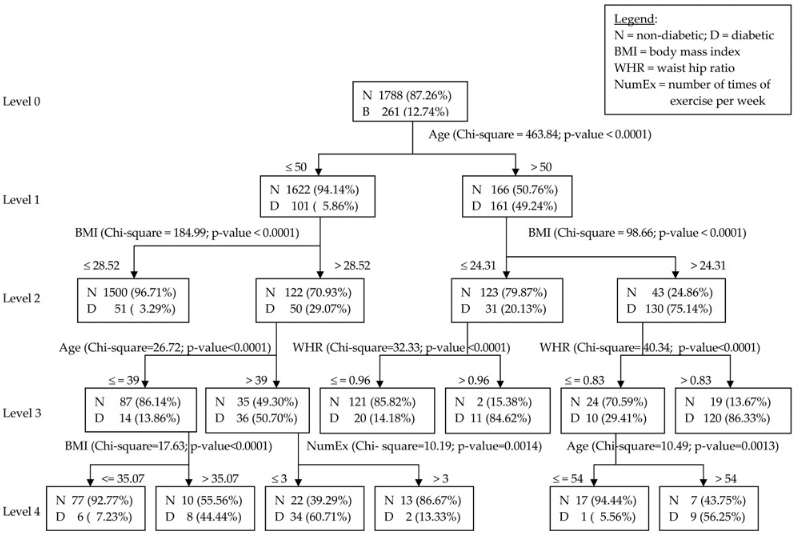
\includegraphics[scale=0.7]{fig/arbol_decision.png}
\linebreak
Figure 1: árbol de decisión\cite{A_DMAHC}
\end{center}
}

\column{0.4}
\block{IMG2}{
\begin{center}
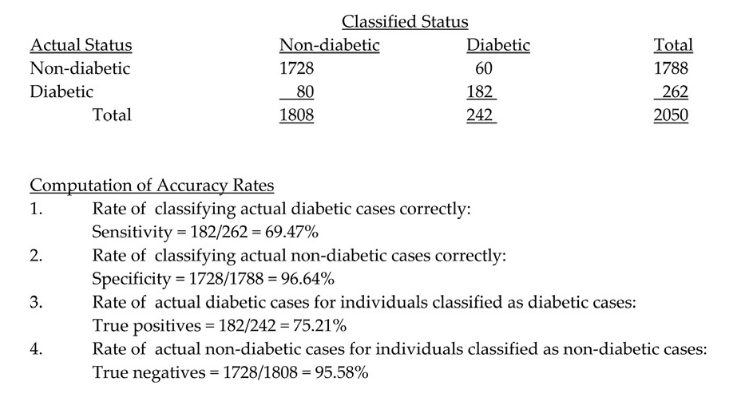
\includegraphics[scale=0.8]{fig/tabla_clasifiacion.png}
\linebreak
Figure 2: tabla de clasificación\cite{A_DMAHC}
\end{center}
}

\column{0.2}
\block{CONCLUSIONES}{
%¿Qué interés tiene en este problema utilizar minería de datos? (¿no hay expertos?, ¿hay demasiados datos?)
%Posibilidad de automatización gracias a abundancia de datos.
Lorem ipsum dolor sit amet, consectetuer adipiscing elit. Etiam lobortis facilisis sem. Nullam nec mi et neque pharetra
sollicitudin. Praesent imperdiet mi nec ante. Donec ullamcorper, felis non sodales commodo, lectus velit ultrices augue,
a dignissim nibh lectus placerat pede. Vivamus nunc nunc, molestie ut, ultricies vel, semper in, velit. Ut porttitor.
Praesent in sapien. Lorem ipsum dolor sit amet, consectetuer adipiscing elit.
}

\end{columns}

\block{}{
\bibliography{bib/bib} 
\bibliographystyle{ieeetr}
}

\end{document}
